\documentclass{article}
\usepackage[utf8]{inputenc}
\usepackage{graphicx}
\usepackage{float}
\usepackage{listings}
\usepackage{color}
\usepackage[english]{babel}
\usepackage{url}
\restylefloat{table}
\definecolor{mygreen}{rgb}{0,0.6,0}
\definecolor{mygray}{rgb}{0.5,0.5,0.5}
\definecolor{mymauve}{rgb}{0.58,0,0.82}



\lstnewenvironment{code}[1][]%
  {\minipage{\linewidth} 
   \lstset{basicstyle=\ttfamily\footnotesize,frame=single,#1}}
  {\endminipage}



\lstset{ %
  backgroundcolor=\color{white},   % choose the background color
  basicstyle=\footnotesize,        % size of fonts used for the code
  breaklines=true,                 % automatic line breaking only at whitespace
  captionpos=b,                    % sets the caption-position to bottom
  commentstyle=\color{mygreen},    % comment style
  escapeinside={\%*}{*)},          % if you want to add LaTeX within your code
  keywordstyle=\color{blue},       % keyword style
  stringstyle=\color{mymauve},     % string literal style
  numbers=left,			   %places line numbers on the left side
}

% Title Page
\title{\project{}: A multi-platform modular test environment.}
\author{Berend van Veenendaal}
\bibliographystyle{plain}
%hieronder wordt de project naam als variabele gedeclareerd
\newcommand{\project}{Codmon-VM}
\newcommand{\CS}{C\nolinebreak\hspace{-.05em}\raisebox{.6ex}{\bf \#}}

\begin{document}
\maketitle

\begin{abstract}
In times when software projects become more and more complex, the testing of this software becomes more and more important. One of the problems with software testing is, that it is difficult to test software in 
different environments. \project{} provides different virtual test environments on which projects can test their software. \project{} is modular, which means that it is easy to add new test cases to the framework 
as well as software components that must be tested. It also provides mechanisms to add new pluggable utility modules to the \project{} environment. The same \project{} version runs on different platforms, so it 
is also multi-platform.
\end{abstract}
\newpage
\tableofcontents
\newpage

\section{Introduction}
\label{sec:Introduction}
This chapter introduces the \project{} project by giving a brief description of the background of my research and of the
previous version of the Codmon project. It also describes the structure of this thesis.

\subsection{Background}
\label{sec:Background}
In times when software projects become more and more complex, testing of this software becomes more and more important. Many software related problems are caused by lack of testing of the 
software~\cite{TTCST}. Typically software is only tested on a single platform, for instance only on a Linux or only on a Windows platform. Setting-up and configuring again and again all 
the different test environments on different platforms simply costs too much time. So, one of the challenges of software testing is to make sure that the software behaves in the same way on 
different platforms, without spending too much time on the installation and configuration of the test environment on these platforms. Even when the test environment is written in such a way 
that it is able to run on different platforms, there are still issues that must be dealt with, before one is able to run and test the software. So in an ideal world we can test the software without being 
worried about setting up the test environment. 

\subsection{Problem indication}
\label{subsec:Problemindication}
Nowdays there are numerous test frameworks and test environments available. For example there is \emph{Junit}\cite{Junit} for Java-unit testing and \emph{NUnit}\cite{Nunit} for \CS{}-unit testing.
There are also different environments like Hudson\cite{HudsonDoc,Hudson}, Jenkins\cite{JenkinsDoc} which can build a project and run a series of (unit) tests against this project. 
These frameworks and environments have both their advantages and disadvantages. One of the advantages of unit testing is that a software developer can easily add new \emph{functional} unit tests.
One of the disadvantages is that standard unit testing ignores non-functional tests like performance testing and the deployment of the software.\\

\noindent Jenkins and Hudson, like Unit tests, also have their
disadvantages. For instance, although they both run on several platforms, in their usage they are not really platform independent. Both Hudson and Jenkins have the possibility to execute shell scripts or 
batch scripts. So, if a user wants to start a test or program he must know in advance on which platform this script has to run. Only then he can decide if he needs a shell script or a batch script. So, although 
this is a powerful feature it is not a 100\% platform independent environment.
 
\subsection{Problem statement}
\label{subsec:Problemstatement}
The test frameworks and test environments mentioned in section \ref{subsec:Problemindication} can be criticized on one or more aspects. What we are looking for is in fact, a combination
of the positive aspects of the described frameworks and environments, without the undesirable aspects. So the central question is, is it possible to design a
multi-platform, modular test environment? In addition, we study if it is possible to design the test environment in a \emph{user friendly} way, meaning that it must
be possible to easily add both new test cases and software without knowing anything about the internal mechanisms of the test environment.\\

\noindent This thesis describes a multi-platform, user friendly modular test environment called \project{}. The \project{} project provides users with a set of virtual machines,
in which \project{} is already installed and preconfigured. The purpose of the virtual machines is to make it easy for users to test software in several environments.  When a user wants to 
test his software on Windows 7, he should download the \project{} windows 7 VM and install it in VM-ware or Virtual box. The same applies for testing his software in an Ubuntu environment. In this case he should 
download the \project{} Ubuntu VM and install this in VM-ware or Virtual box. By doing it this way the  only tasks a user of \project{} has to do are 1) add their project to an initialization file and 2) add 
the tests to a so called wrapper file. This will be discussed in more detail in section \ref{sec:Codmon2.0}.


\subsection{Thesis outline}
\label{subsec:Thesisoutline}
Section \ref{sec:codmon} first describes the original Codmon framework and the motivation for its development. It also identifies its shortcomings. In section \ref{sec:road}, \emph{The road to \project{}}, 
we explain how we got to the final \project{} design. Section \ref{sec:Codmon2.0} describes the implementation of the \project{} project. 
It starts with a general description of the project followed by a detailed explanation of the different modules of \project{}. In section \ref{test} we discuss some tests we've executed on different platforms 
with \project{}. Next we evaluate the choices and their consequences in section \ref{sec:evaluation}. In Section \ref{sec:future} we discuss the results based on section \ref{sec:evaluation}. We end 
this section with a brief discussion of related work.

\newpage
\section{Codmon}
\label{sec:codmon}
In this section we describe the original Codmon framework and its shortcomings. The original Codmon framework was built in 2005 by François Lesuer\cite{Codmon}. Originally Codmon was built for 
testing and performance monitoring Ibis projects\cite{Ibis,Satin,MPJ,IPL,GMI} on the DAS-2\cite{das2} computer. Codmon was able to perform both functional and performance tests.\footnote{At 
this moment both the DAS-2 and Codmon are not in use anymore.} If for some reason a particular test fails, Codmon raises an alarm and reports the failures. Codmon does so by 
sending an email directly to the programmer who made the last changes in the software that was tested. Codmon also reports in the same way in case the measurements change significantly. 
Next to sending an email in case of failing tests, Codmon also presents the results on a web page. It was also the intention that Codmon would be extensible. In this the Codmon programmers 
succeeded only partially. We will discuss this more in depth in section \ref{subsec:CodmonProblems}.  

\subsection{The working of Codmon}
\label{subsec:CodmonDesign}
In this section we will describe the design of the Codmon framework. The Codmon framework is more or less modular and consists of two parts: the part that controls Codmon and the Codmon core program.\\

\subsubsection{Controlling Codmon}
\label{control}
\noindent We first describe the part that controls Codmon. With controlling we mean which test will run and in which order they will run. There are two different kinds of tests, functional and non-functional 
tests. The source code of the projects that will be tested is stored in a \emph{CVS} repository. Both the functional and non-functional tests are described in so called \emph{sensor} files. A sensor file 
describes a "test set" that can be executed by the Codmon program. Such a sensor file consists of two parts. First there is the \emph{onoff} part, which is used for functional tests. This includes the compilation 
of the software, which is a special kind of functional test. These tests can either fail or succeed. Second there is the \emph{graph} part. This part is used for the performance tests. Each test of such a test 
set is described by a \emph{sensor-element}. The core of each sensor-element in a sensor file is the CMD attribute. This CMD attribute consists of two basic parts: a wrapper and a shell-script command. 
This shell-script command can be anything. For instance it can be a SVN command, or a ANT job or something else. Listing \ref{list:sensor} gives an example of such a sensor.\\


\lstset{
  captionpos=b,
  caption = \emph{Sensor example},
  label =list:sensor
}
\begin{code}[frame=shadowbox, language=XML,showstringspaces=false]
 <sensor id="update_ok" 
    name="CVS update" 
    cmd="perl CODMON_HOME/codmon/wrappers/time_wrapper.pl CODMON_HOME sh codmon/local/cvsup.sh" 
    scope="ibis" 
    scheduled="false"
    enabled="true"
    graph="true" 
    fatal="true" />
\end{code}

\noindent In this case the CMD attribute apparently consists of a wrapper called \emph{time\_wrapper.pl} and a shell-script command called \emph{cvsup.sh}. The wrapper indicates the kind of test
that is executed. The shell-script command indicates which program is tested. In the case of Listing \ref{list:sensor} the update time of the CVS repository is is measured. Table \ref{tab:codsensor} describes
the attributes of a sensor\cite{Codmon}.\\

\begin{table}[h]
\centering
  \begin{tabular}{ | l| p{5cm} |}
  \hline
  \textbf{id} & Unique ID of the sensor. \\ \hline
  \textbf{name} & Name of the sensor. \\ \hline
  \textbf{cmd} & Command to be ran, eventually inside the wrapper. \\ \hline
  \textbf{scope} & The repository folder which should be analyzed in case of an alarm. \\ \hline
  \textbf{scheduled} & Whether this sensor is scheduled downward. If true jobs will be launched in parallel, letting the system care about the real scheduling. \\ \hline
  \textbf{enabled} & Whether this sensor is enabled. If true the sensor will be run. \\ \hline
  \textbf{graph} & Whether this sensor is to be graphed. If true, a time graph will be generated. \\ \hline
  \textbf{fatal} & Whether failing in this step is fatal. If true, no further tests should be executed.\\ \hline
  \end{tabular}
\caption{Table 1: Codmon sensor}
\label{tab:codsensor}
\end{table}


\noindent Where a \emph{sensor} describes the structure of a set of tests, a so called \emph{wrapper} describes the actual test. Wrappers are small programs that are written in the PERL
language. The return value of a wrapper indicates if a test was successful or not. In case of a failure an alarm is raised and both the return value and the actual error code will be mailed to
the programmer who made the last contribution to the code.\\

\noindent It is fundamental to understand that a \emph{wrapper} is not part of the Codmon program itself. Leaving the wrappers outside of Codmon gives a user the possibility to add their own 
wrappers as well as using general wrappers without knowing the the details of the actual Codmon program. A general wrapper is a wrapper that can be used for each software component. The 
\emph{time\_wrapper} is a good example of a general wrapper. The time\_wrapper measures the duration of a test. This can be very useful to see if changes to the program that is tested have influenced the 
duration of a test. This duration can give an indication if the performance of the software has changed. Figure 1 shows a schematic picture of the Codmon structure \cite{Codmon}. More technical details 
about the Codmon implementation can be found in \cite{Codmon}.\\

\begin{figure}[!ht]
  \caption{\emph{Codmon}}
  \centering
    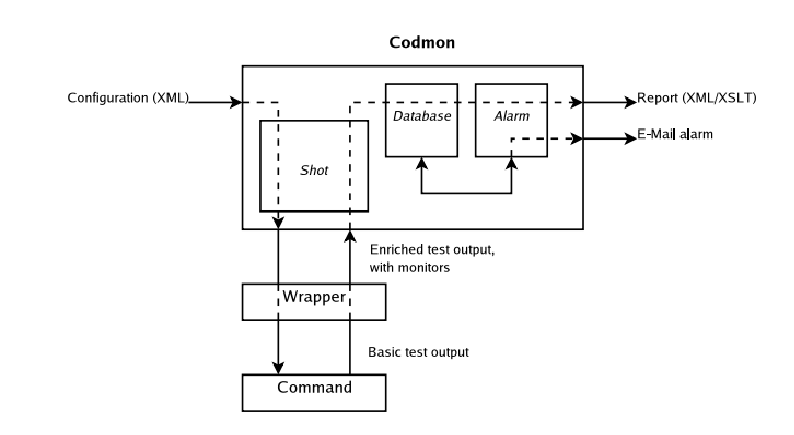
\includegraphics[scale=0.5]{codmon}
\end{figure}

\subsubsection{The Codmon core program}
\label{coreprogram}
\noindent When a user wants to test one of the applications mentioned above, the only thing he must do is to make sure that the Codmon framework is installed on the Das-2. He needs to know nothing of the 
Codmon program, except for how it should be started. The \emph{core-part} of Codmon is responsible for a few things. First it creates a \emph{shot} of the actual state of the programs that are 
tested. It does this by \emph{periodically} executing a set of \emph{sensors} and collecting the output of these executions. In case of a performance test (the sensor file will make the distinction between 
functional test and a performance test) the test information is stored in a RRD database\cite{RRD}. From this data, averages are calculated and eventually the graphs are generated\cite{Codmon}. The results 
of a performance test will be compared with the results of previous tests and if the performance result of a test changes significantly, an alarm is raised. When an alarm is raised, an email is sent 
to the last contributor to the tested code. The same happens when one or more functional tests fail.\\
 

\subsection{Codmon problems}
\label{subsec:CodmonProblems}
The goal of this research was to see if it's possible to design a multi-platform, user friendly modular test environment. There are multiple reasons why Codmon does not fit the bill. In this section
we'll discuss these reasons in detail.
 
\subsubsection{Multi-platform}
\label{prob:multi}
First of all, Codmon is not multi-platform. To be multi-platform, without applying every change multiple times, Codmon itself must be written in a platform-independent language. 
In Codmon, at least three different languages are used. The Codmon program itself is written in Java, which is indeed platform independent\cite{Java}, so this is not the real problem. As we've explained in 
section \ref{subsec:CodmonDesign}, the core-part of the sensors is a combination of a \emph{shell-script} command and a \emph{wrapper}. Since a Unix shell-script usually won't work in a Windows environment 
this part is definitely not platform independent. The same can be said about the PERL language; this will, without special effort, also not work in a Windows environment. Next to this there are also several 
separate shell-scripts, for example for  CVS-checkouts and the startup of the Codmon framework. Taking this into account, we can easily see that the Codmon framework is far from platform independent.

\subsubsection{Modularity}
\label{prob:modular} 
The second reason why Codmon doesn't fit the bill, is the modularity in Codmon. Due to the chaos of different scripts and languages it is difficult for programmers to add new modules or tests to the Codmon 
framework. Adding new tests and modules should be straightforward. 

\subsubsection{User-friendliness}
\label{prob:user}
The third problem is the user-friendliness of Codmon. Next to modularity, which also contributes to the user-friendliness of the test environment, Codmon requires quite a bit of configuration before it can 
be used. In the remainder of this thesis we'll explain in detail how we have solved these and other issues in the \project{} environment.\\
 
\noindent Another issue concerning user-friendliness is the structure of the wrappers. As discussed in section \ref{subsec:CodmonDesign}, the CMD attribute of a sensor consists of two basic parts: 
a wrapper and a shell-script command, of which the shell-script command could be anything. From a users perspective it would be much easier if there was only one type of command possible, an Ant-job\cite{Ant} 
for instance.\\

\noindent A third issue regarding user-friendliness is the limited support of version control systems. Codmon only supports \emph{CVS}\cite{CVS}. From a user-friendliness perspective it would be much better 
if Codmon would support multiple version control systems, for instance SVN\cite{SVN} or Git\cite{Git}. It also would be nice if other version control systems could be easily added to the test environment.


\section{The road to \project{}}
\label{sec:road}
As we described in section \ref{subsec:Problemstatement} our goal is to develop a test environment that must at least satisfy the following requirements:

\begin{itemize}
\item \project{} should be \emph{multiple-platform}, which means that the same source, without making any modifications, can compile and run on multiple platforms.
\item \project{} should be \emph{modular}, which means that it must be possible for users to easily add new components to the environment. The same should apply to developers who maintain the environment.
\item \project{} should be \emph{user-friendly}, which means that we don't want to bother the users of the \project{} environment with its internal mechanisms. Also, the sensors as described in 
section \ref{subsec:CodmonDesign} should all have the same structure so a user can add tests always in the same way.
\end{itemize}

\subsection{General decisions}
\label{subsec:general}
In the previous sections we have stated that Codmon has some good aspects as well as some aspects that aren't that good. For our new test environment we decided to reuse the good parts of Codmon and design 
new components where necessary to fulfill the requirements described above. Since the core program of Codmon is written in Java and Java is multi-platform we decided to reuse most of this code and to 
modify it where needed. In section \ref{sec:Codmon2.0} we show where, how and why we adapted the Codmon core program. 

\subsection{Multi-platform}
\label{road:multi}
Because the Codmon core program is written in Java already we decided to write the all wrappers in Java as well. Using as few languages as possible will help in maintaining the environment. 
We also saw that in the original Codmon framework the core of a sensor consists of two parts: a wrapper and a shell-script command. In most cases this shell-script command will start some 
program. This program should also be able to run on multiple platforms, so writing these programs in Java as well is an obvious choice. So now we have a Java wrapper and a Java program. We thus need a 
multi-platform construction that, at least, is able to start a program. We have chosen to use \emph{Ant} for this. The main reason to choose Ant is that it provides us with a lot of flexibility. Lets take 
a look at the following example. A user who wants to test a piece of Java software probably already has a build file for building the software. So there is nothing new here. The only thing the user has 
to add is a new ant-target, which starts the program. Listing \ref{list:sensorNew} shows an example of the new sensor structure.

\lstset{
  captionpos=b,
  caption = \emph{Sensor new structure},
  label =list:sensorNew
}
\begin{code}[frame=shadowbox, language=XML,showstringspaces=false]
 <sensor id="update_ok" 
    name="CVS update" 
    cmd="java <wrapper> <relative path to build file> <ant target>" 
    scope="ibis" 
    scheduled="false" 
    graph="true" 
    fatal="true" />
\end{code}

In section \ref{sec:Codmon2.0} we'll show how this all is implemented in the \project{} environment. The key idea is that all software that is to be tested is started by invoking Ant.\\

\subsection{Modularity}
\label{road:modular}
Another problem we discussed in section \ref{subsec:CodmonDesign} is the modularity of the environment. The way Codmon was designed it could only handle CVS-checkouts and updates. The \project{} 
environment must be able to deal with different version control systems. To achieve this goal we decided to design separate \emph{modules} outside of the \project{} core program to take care of the checkouts and updates of the 
software that the users want to test. Each of these modules implement the \emph{versionControl} interface for a different version-control system.
This interface defines mechanisms for fetching and updating the software.
Next to this it 
also provides a basic mechanism to obtain the history log of the software.
Listing \ref{list:interface} shows the versionControl interface.
Adding support for a new version-control system implies that the codmon developers 
(or the users of \project{}) have to write a new module that implements this interface for this new version-control system.
The user only has to indicate which version control system his 
software is using. We discuss the implementation in more depth in section \ref{sec:Codmon2.0}.\\

\lstset{
  captionpos=b,
  caption = \emph{VersionControl interface},
  label =list:interface
}
\begin{code}[frame=shadowbox, language=Java,showstringspaces=false]
/**
@author bvl300 
Basic interface for version control modules
*/
public interface VersionControl{
	
	/**
	*Fetches a repository
	**/
	public void update() throws VersionControlException;
	
	/**
	*If there is no log file it creates the log file. 
	*If there is a log file it updates the existing log file
	**/
	public void updateLog() throws VersionControlException;


	/**

	*Returns the revision nr of the last commit.
	*Because this doesn't make sense for all version control
	*system it may throw a MethodNotSupportedException.

	**/
	public long getRev() throws MethodNotSupportedException;
}
\end{code}


\subsection{User-friendliness}
\label{road:user}
When a user wants to test his software on multiple platforms he does not want to download, install and configure the test environment over and over. The \project{} project comes up with a nice and powerful 
solution for this problem. It provides the user with a set of virtual machines in which \project{} is already installed en pre-configured. When a user wants to start using the \project{} environment he only 
has to do the following steps.

\begin{itemize}
\item Download one or more of the \project{} VM's.
\item Install them into VM-ware or Virtual box.
\item Add the details of the software he wants to test to the initialization file.
\end{itemize}


\noindent Now the nasty configuration details are hidden for the users of the \project{} environment. Also when a a new version of an operating system arrives, the \project{} developers only have to 
configure one new image, which is directly available for all the users. How this works exactly we'll see in section \ref{sec:Codmon2.0}. \\

\noindent Another issue concerning user-friendliness is the one of adding new tests to the sensor file. As discussed in section \ref{road:multi} adding new tests is also straightforward. All a \project{} user 
has to do is add a new test to the Sensor file, and create an Ant target for this test. 

\newpage
\section{The implementation of \project{}}
\label{sec:Codmon2.0}
In this section we'll describe how we've implemented the decisions made in section \ref{sec:road} in the \project{} project. We'll start with the parts that were necessary to achieve that \project{} is multi-platform 
followed by the parts concerning the modularity of \project{}. We end this section with the parts that provide user-friendliness. When someone wants to use the \project{} test environment there are two options  
to get access to this environment. We'll come to these options later in this section. For now we assume the user has access to a working \project{} environment.

\subsection{Multi-platform}
\label{imp:multi}
In the previous sections we mentioned that the tangle of shell-scripts and PERL-code ensures that Codmon isn't multi-platform. To ensure that \project{} is multi-platform we chose to implement the 
\project{} environment completely in Java. First we describe how we implemented the initiation of a test run. Then we describe how both the tests and the software that is tested are connected together.

\subsubsection{Initialization}
\label{imp:start}
In a single-platform environment it is very easy to create a shell-script (or a batch-file in case of Windows) to start a program. In Java, this is a little more complex.\\

\noindent In section \ref{imp:modular} we describe that everything outside the \project{} core program is a separated module, including the start-up module. The start-up module is called with one parameter: 
the name of the sensor file that describes the tests that will be executed in this run. The start-up module is responsible for several tasks. First it initializes the \project{} environment. If it is the 
first time \project{} is used, four result folders are created: Three history folders and a "current result" folder. Otherwise the results of the previous test-runs are copied to history folders so the 
current result folder, called \emph{dday}, has space for the new test results \footnote{For historic reasons the result folders are called dday,dday1,dday2 etc.}.\\

\noindent When all the result files of the previous tests are copied to the history folders the \project{} core program can be started. To increase the modularity of \project{} this is done dynamically, so 
it is possible to start different programs with the same StartUp module. Because this is a completely new Java program we needed a way to pass the sensor file parameter to the core program. Remember at 
compile it is unknown which program has to be initiated. So to achieve this we have to make use of \emph{dynamic class loading}. Dynamic class loading means that which (Java) class is called is determined 
at runtime. Listings \ref{list:method} and \ref{list:run} in Appendix \ref{AppendixA} show how this is implemented in the \project{} environment.


\subsubsection{Ant-connector}
\label{imp:ant}
A second issue we had to deal with were the sensors in the sensor files. In section \ref{road:multi} we have already seen the new sensor structure. A wrapper is a separate process which has to be started by 
the \project{} core program.  When the \project{} core program evaluates a sensor it first extracts the wrapper from the sensor \emph{cmd}-attribute. Then the Ant-target is extracted from the 
\emph{cmd}-attribute. If we use the sensor of listing \ref{list:imp_sensor} the wrapper will be the \emph{TimeWrapper}, while the Ant-target will be \emph{"run"}.\\

\lstset{
  captionpos=b,
  caption = \emph{sensor example},
  label =list:imp_sensor
}
\begin{lstlisting}[frame=shadowbox, language=XML,showstringspaces=false]
<sensor id="checkout_ok" name="TestApps: checkout projects" 
  cmd="java CODMON_HOME/codmon/wrappers/classes/TimeWrapper ../../local/checkoutApplications run"  
  scope="checkOut" 
  scheduled="false" 
  graph="true" 
fatal="true"/>
\end{lstlisting} 

\noindent When the \project{} core program has extracted these values it starts a \emph{Wrapper} process (See appendix \ref{AppendixC}). Listing \ref{list:process} shows how this is done. The Ant target is 
passed as a parameter to this Wrapper process. This Wrapper, which is a test, starts he Ant-connector, which is a small Java Class (see Appendix \ref{AppendixC}) which evaluates and executes the Ant-target. 
Such an Ant-target can be a "simple" \emph{build} target or in this case it is the \emph{run} target. This is shown in listing \ref{list:runTarget}. This "run"-target executes the software that is tested by, 
in this case, the TimeWrapper.\\
 

\lstset{
  captionpos=b,
  caption = \emph{Start a new process: The different elements of the CMD attribute of the sensor described in listing \ref{list:imp_sensor} are separately stored in the \emph{argList} argument. The dir argument 
indicates the location from where the process should start},
  label =list:process
}
\begin{lstlisting}[frame=shadowbox, language=Java,showstringspaces=false]
final Process pr = new ProcessBuilder(argList)
 		 .directory(new File(dir)) 
    		 .start();
\end{lstlisting} 


\lstset{
  captionpos=b,
  caption = \emph{The run-target},
  label =list:runTarget
}
\begin{code}[frame=shadowbox, language=XML,showstringspaces=false]
	<!--Run the Checkout program-->
	<target name="run">
		<java  fork="true" classname="Checkout" classpath="${env.CLASSPATH}" output="out.txt">
	  		<classpath>
				<path location="${jar.dir}/CheckoutApplications.jar"/>
	        	</classpath>
			<arg value="${arg0}" />
			<arg value="${arg1}" />
		</java>
	</target>
\end{code} 

\noindent By implementing it this way it doesn't matter which (Java-)software\footnote{Theoretically it is also possible to run non-Java applications, but they are out of scope for the \project{} project. 
See also section \ref{sec:future}.} the wrapper wants to test, it will always be done in the same way as described above.


\subsection{Modularity}
\label{imp:modular}
In section \ref{imp:multi} we described the improvements we made to achieve that \project{} is multi-platform. In this section we'll describe how easy it is to add new modules to the \project{} environment. 
To do this we use a module called \emph{CheckoutApplications}.


\subsubsection{CheckoutApplications module}
\label{imp:checkout}
Before \project{} is able to test any software, this software must be available for the \project{} environment. To be available this software must have been extracted from the repository where it is stored. 
The CheckoutApplications-module is responsible for this job. The CheckoutApplications itself consists of a main checkout module and different sub-modules which support a specific version control system. 
Currently, the CheckoutApplications module supports two different version control systems, namely Subversion (\emph{SVN}) and Git.\\

\noindent
The main checkout module is responsible for several tasks. First it reads the initialization file, which contains information about the test projects. We'll come back to the initialization file later. This 
information contains, among others, the kind of version control system that is used for this software. With this information both the update and updateLog methods for this software can be invoked (See 
Appendix \ref{AppendixD}). For implementing these methods for SVN repositories we've used the \emph{SVNKit} Api\cite{SVNKit}. For the Git repositories we've used the \emph{JGit} 
Api\cite{JGit}.\\

\noindent For a user, now it is easy to add a sub-module for a new kind of version control system. The only thing a developer has to do is add a module that implements the update and updateLog methods
for this version control system, and add an instantiation of this module
to the \emph{checkoutProject} method shown in Appendix \ref{AppendixD}. The \emph{update} method is responsible to check if the latest version of the software is locally available for 
testing. If this is not the case it does a checkout or update on the software's repository. The \emph{updateLog} method is responsible for maintaining the log file of the software. 

\subsubsection{Tests}
\label{imp:tests}
Adding new tests is relatively straightforward. As long as the test is written in Java a user can just add a reference to this test to the CMD-attribute of a sensor. This works the same way for both functional 
and non-functional tests.


\subsection{User-friendliness}
\label{imp-user}
Finally it's time to discuss the user-friendliness of \project{}. As we said before, we don't want to bother the \project{} users with its internal mechanisms. Neither do we want to bother them with 
its time consuming configuration. This section describes why \project{} is a very user friendly environment.\\

\subsubsection{The initialization file}
\label{imp:init}
\noindent Before the \project{} environment is able to run one or more tests on a software, it has to know where it can find this software and extract it from its repository. This information and other information has to be added to 
the \emph{initialization file}, which is an XML file. Listing \ref{list:init} shows the structure of this initialization file. The explanation of its elements is shown in table \ref{tab:init}. \\

\lstset{
  captionpos=b,
  caption = \emph{Initialization file},
  label =list:init
}
\begin{lstlisting}[frame=shadowbox, language=XML,showstringspaces=false]
 <projects>
	<project>
		<name>projectname</name>
		<location>http://www.sampleurl.com</location>
		<versionControl>
			<type>svn</type>
			<command>checkout</command>
		</versionControl>
		<run>true</run>
		<user>username</user>
		<pwd>pwd</pwd>
	</project>
</projects>
\end{lstlisting} 


\begin{table}[ht]
\centering
  \begin{tabular}{ | l| p{5cm} |}
  \hline
  \textbf{projects} & List of all the projects that are involved in a test series. \\ \hline
  \textbf{project} & Contains the information of a specific project. \\ \hline
  \textbf{name} & The name of the project. \\ \hline
  \textbf{location} & The URL of the location where the project can be found. \\ \hline
  \textbf{versionControl} & Element that contains specific information about the version-control system \\ \hline
  \textbf{type} & The type of version control system that is used for the project. e.g. \emph{SVN} or \emph{Git} \\ \hline
  \textbf{run} & \textbf{Boolean} that indicates if a project should be tested. \\ \hline
  \textbf{user} & username to login into the version-control system \\ \hline
  \textbf{pwd} & password to login into the version-control system \\ \hline
  \end{tabular}
\caption{Elements of the initialization file. In Section \ref{sec:evaluation} and section \ref{sec:future} we'll come back to the security issues regarding the user name and password}
\label{tab:init}
\end{table}


\noindent The only tasks that are left for a user  when he wants to test a new software component is adding a new project to the initialization file, create a new sensor file for it and add a run-target 
to the software's build file (See Appendix \ref{AppendixE}.). When a user wants to use or create his own tests he must create its own wrapper(s) for this.\\ 

\noindent There is only one issue left that we have to mention here. The initialization file contains two fields, namely \emph{user} and \emph{pwd}. For this thesis it is OK to do it this way, but in real life 
this would be a security risk. 

\subsubsection{Virtual environments}
\label{imp:virual}
We have said already a few times that we don't want to bother the users of the \project{} environment with its configuration. We came up with the idea that it would be nice and extremely useful if a 
user just use a preconfigured \project{} environment. To achieve this the \project{} project provides a set of virtual machines on which \project{} is already installed and preconfigured. The only thing a 
user must do is install VM-ware (or Virtual box), download one of the provided \project{} images and install them in VM-ware.\\

\noindent The developers of the \project{} can easily provide new images, by installing a \emph{"clean"} image of the target platform, Windows or one of the different Linux distributions for instance, and 
install and preconfigure \project{} in this image. When this is done successfully, VM-ware provides options to create a new distributable image of the preconfigured environment. 

\newpage
\section{Testing \project{}}
\label{test}
In this section we describe how we have tested \project{} with an independent Java project.

\subsection{Test preparation}
\label{test:prep}
For testing \project{} we chose to use the \emph{Marc4j}\cite{marc4j} project. There were a few criteria for choosing a test project:

\begin{itemize}
\item It must be a \emph{Java} project.
\item The project must contain a build.xml.
\item It should be a 3\textsuperscript{rd} party project.
\end{itemize} 

\noindent To find a project that met the requirements described above, we browsed the \emph{Github}\cite{Github} repository. Eventually we found the \emph{Marc4j} project which satisfied our criteria.\\

\noindent After choosing a suitable test project we had to decide on which platforms, we should test this software. To show that \project{} runs on multiple platforms we decided to test the \emph{Marc4j} 
project both on a \emph{Windows 7}-environment and on a \emph{Ubuntu 11.10}-environment.\\

\noindent Now that we have chosen a test project and two different platforms to execute the tests, we had to decide which tests we should execute. To cover both functional and non-functional tests we 
decided to use the TimeWrapper for the non-functional tests. This TimeWrapper measures the execution time of a piece of software. For the functional tests we used the JUnit tests of the \emph{Marc4j}-project 
itself. To test an error situation we added one test that always fails.\\

\noindent Finally we decided to have the tests executed by someone who's not involved in the \project{} project\footnote{The tests are executed by H.J. van Veenendaal.}.

\subsection{Test execution}
\label{test:exec}
Before we could test the software, we first had to add the \emph{Marc4j} project to the init file (listing: \ref{list:test:init}) and to a sensor file (listing: \ref{list:test:sensor}). The tests that are 
used in the sensor file measure both the checkout and build time of the \emph{Marc4j} project. There are no credentials needed for checking out the \emph{Marc4j} project so both the \emph{user} and 
\emph{pwd} fields in listing \ref{list:test:init} could be left empty. The last sensor runs the Marc4j JUnit-tests.\\

\noindent Now that we have configured the tests, they are ready for execution. We decided to run the whole set twice. The first time they run without errors. The second time we've added a ErrorTest to 
project's JUnit-test set.The results are shown in the next section.

\lstset{
  captionpos=b,
  caption = \emph{Initialization file for testing the Marc4j project},
  label =list:test:init
}
\begin{code}[frame=shadowbox, language=XML,showstringspaces=false]
 <projects>
	<project>
		<name>Marc4j</name>
		<location>https://github.com/marc4j/marc4j.git</location>
		<versionControl>
			<type>git</type>
			<command>clone</command>
		</versionControl>
		<run>true</run>
		<user />
		<pwd />
	</project>
</projects>
\end{code} 

\lstset{
  captionpos=b,
  caption = \emph{Sensor file for testing the Marc4j project},
  label =list:test:sensor
}
\begin{code}[frame=shadowbox, language=XML,showstringspaces=false]
<?xml version="1.0" encoding="ISO-8859-1"?>
<?xml-stylesheet type="text/xsl" href="libs/style.xml"?>

<sensors>
	<onoff>	
		<!-- check out the  projects-->
		<sensor id="checkout_ok" name="TestApps: checkout projects" cmd="java CODMON_HOME/codmon/wrappers/classes/TimeWrapper ../../local/checkoutApplications ant run"  scope="checkOut" scheduled="false" graph="true" fatal="true"/>
	
		<!--Build the Marc4j project-->
		<sensor id="build_marc4j_ok" name="TestApps: build Marc4j" cmd="java CODMON_HOME/codmon/wrappers/classes/TimeWrapper ../../../marc4j ant dist" scope="testApps" scheduled="false" graph="true" fatal="true"/>
	
		<!--Run Marc4J unit tests-->
		<sensor id="test_marc4j_ok" name="TestApps: test  marc4j" cmd="java CODMON_HOME/codmon/wrappers/classes/TimeWrapper ../../../marc4j ant test" scope="marc4j" scheduled="false" graph="true" fatal="true"/>
	</onoff>

	<graph>
	</graph>
</sensors>
\end{code}

\newpage
\subsection{Test results}
\label{test:results}
During the execution of the tests we ran into one small issue. The Ant-connector expects the default build target to be named \emph{"main"}, in case of the \emph{Marc4j} project this was not the case. This 
issue was easy to fix by adding the expected target to the \emph{cmd}-attribute of the sensor, but is something to keep in mind. Because the test executions on the \emph{Windows} and the \emph{Ubuntu} 
environment gave similar results, we only show the results of the \emph{Windows} environment. The results of the three tests described in section \ref{test:exec} are shown in figure 2 and 3. 
Figure 2 shows the results of the run without errors on a screenshot from a browser page, which is generated by the \project{} environment. Figure 3 shows the same page, but in this case the ErrorTest is 
included in the test set\\

\begin{figure}[!ht]
  \caption{\emph{Test results without errors}}
  \centering
    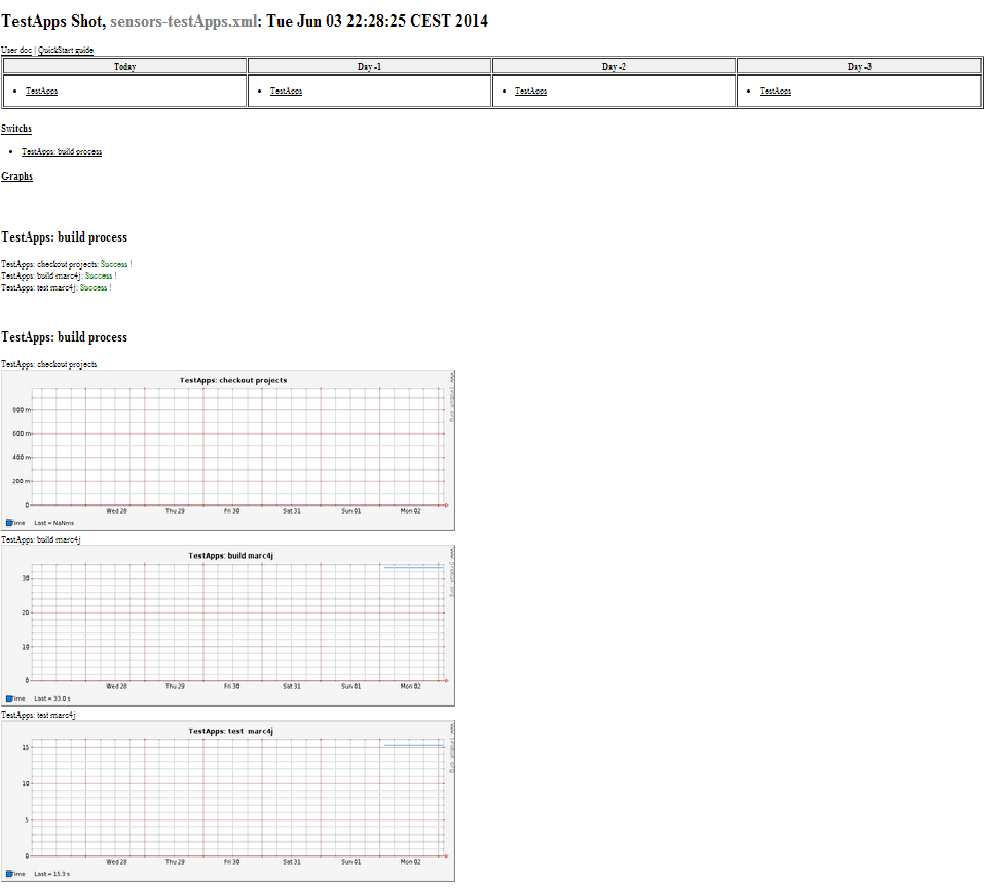
\includegraphics[scale=0.5]{testResultsGood}
\end{figure}


\begin{figure}[!ht]
  \caption{\emph{Test results including an error}}
  \centering
    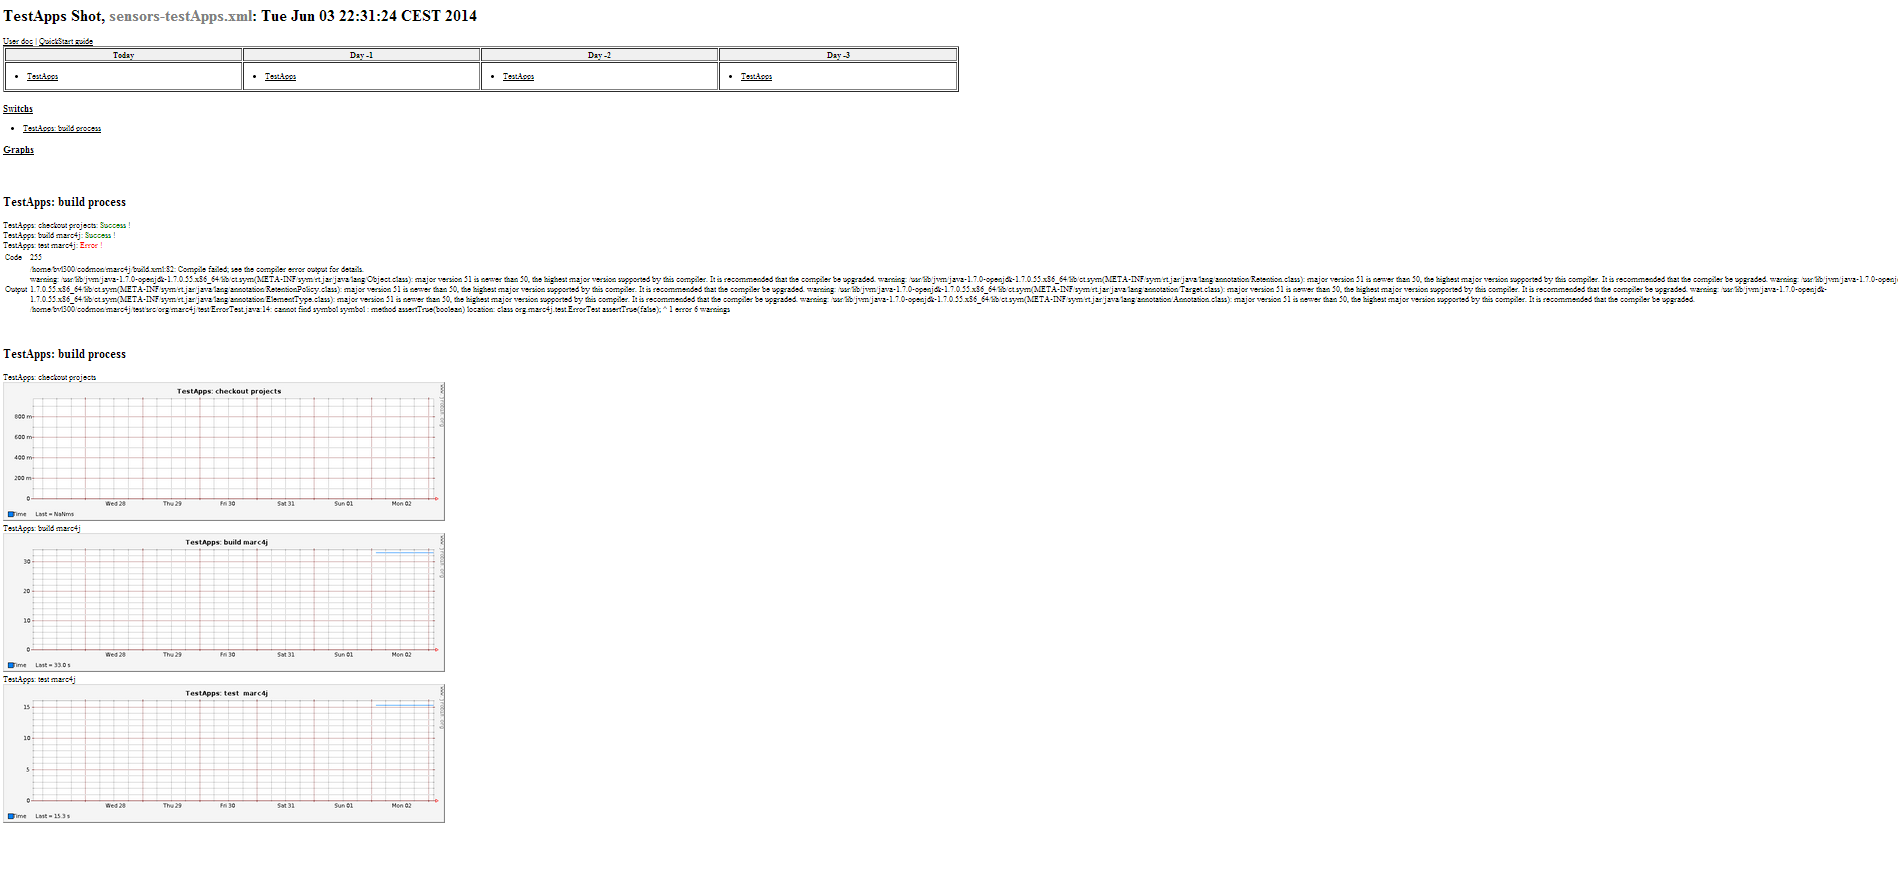
\includegraphics[scale=0.5]{testResultsError}
\end{figure}

\newpage
\noindent The page displays several elements. On top of the page urls are shown which navigate you to the historical results. As you can see in figure 3, in case of an error also the error message is 
displayed. Finally a list is shown, giving an overview of the executed tests. In this case the executed tests were:

\begin{itemize}
\item TestApps: checkout projects.
\item TestApps: build marc4j.
\item TestApps: test marc4j.
\end{itemize}

\noindent Below this list the graphs are shown with the results of the \emph{timeWrapper} test.

\newpage
\section{Discussion and Conclusion}
\label{sec:evaluation}
In section \ref{subsec:Problemstatement} we proposed the following question: \emph{"Is it possible to design a multi-platform, modular test environment"}? In addition, we've studied if it would be 
possible to design such a test environment in a user-friendly way, meaning that it must be possible to easily add both new test cases and software without knowing anything about the internal mechanisms of this test environment. 
In section \ref{sec:road} and \ref{sec:Codmon2.0} we showed that, at first sight, the answer to these questions can be answered with yes. Before making that our final conclusion let's first take a deeper look 
into what we have a achieved and discuss the pros and cons of \project{}. \\

\subsection{Multi-platform}
\label{dis:multi}
Let's first take a look at the multi-platform requirement. A software program or environment is considered to be multi-platform \emph{when it is compatible with or involving more than one type of computer or 
operating system}\cite{def:multi}. This means that \project{} must be able to run on multiple platforms and that its runtime behavior is the same on these platforms. To achieve this we built the whole 
\project{} environment, in contrast to the Codmon framework, in the Java programming language. To connect the different Java components we made use of Ant. By doing this, at least we are sure \project{} 
runs on multiple platforms\cite{Java}.\\

\noindent That \project{} runs on multiple platforms doesn't mean that the runtime behavior is also the same on these platforms. To see that the runtime behavior must be the same on these platforms we created 
different images of \project{}, both Windows and Linux. Running the same tests in these images showed us that the runtime behavior is also the same on these platforms (See Section \ref{test}). So we can 
conclude that \project is a \emph{multi-platform} environment.\\


\subsection{Modularity}
\label{dis:modular}
The second requirement we have to discuss is the modularity of the \project{} environment. This is a little less straightforward than the Multi-platform requirement. The main question we have to answer is: 
\emph{when do we consider the environment to be modular?}. Is it modular if a user of the environment can add new tests in a straightforward manner? Is it modular when it is easy to add new, or extend, utility 
modules like the checkout Applications module? Or is \project{} environment only modular if the core program itself is modular as well? To answer this question we have to consider what the main purpose of the 
\project{} environment is. When we summarize all the requirements we can see that the environment should be especially easy to use and maintain. This brings us nothing further. What do we mean by 
maintenance? Are we talking about the \project{} core program or about adding (and removing) functionality and tests?

\noindent When we only take the modularity regarding to usage and maintenance of the environment into account and not that of the \project{} core program, \project{} is also \emph{modular} (See Section \ref{test}). 
When we take the \project{} into account it's only partially modular.\\

\subsection{User-friendliness}
\label{dis:user}
Where in section \ref{dis:multi} the question was straightforward and in section \ref{dis:modular} the discussion was only about two different viewpoints, the subject of user-friendliness is even more complex. 
Where one person might say it is user-friendly when the environment is quick and easy to use, another person might say that an environment is only user-friendly when is has a nice and fancy user interface.\\

\noindent Let's first look at how easy the \project{} environment is in its usage. The user can easily download a \project{} environment image and install this in VM-ware or Virtual box. When this is done, 
\project{} is immediately ready for usage. In sections \ref{imp:modular} and \ref{test} we also showed how easy it is to add new tests and (utility) modules like the checkoutApplications module. So when we only take this into 
account we can conclude that the \project{} environment is user friendly.\\

\noindent Now let's take a look at the second issue. Earlier we've described mechanisms for both adding new software that should be tested, as well as adding tests to a sensor file. The only difficulty 
some users could have with it is that they directly have to edit XML files. Doing this, using a nice and fancy user interface could improve the user-friendliness of \project{}. Also, adding both to be 
tested software and new sensors via a graphical user interface will reduce the risk of errors in these files. Such a user interface could also be used to display the test results. Doing it this way, 
\project{} would appear as one coherent environment to its users.\\

\noindent So looking at the \emph{user-friendliness} of \project{} it depends on the person how he or she thinks about user-friendliness. But one thing we can certainly say about \project{}: the possibility of 
preconfigured virtual machines and the way of adding new to be tested software, sensors and utility modules definitely offers some user-friendliness!

\newpage
\section{Future work and Recommendations}
\label{sec:future}
Finally we describe what future work and research, regarding to \project{}, could be done to improve it. When we take a look at what we've described in sections \ref{dis:modular}
we see that the \project{} core program is still one big monolithic program. To improve the maintainability of \project{} it would be useful to see if and how we can transform this monolithic 
program into a program with a more modular design.\\

\noindent In section \ref{dis:user} we described different views on user friendliness. In our opinion the biggest improvement could be gained with a nice and fancy user interface. It would 
really worthwhile to see if it is possible to combine \project{} with a tool like Jenkins \cite{JenkinsDoc}. Jenkins could probably provide a user interface to at least start tests that use 
different sensor files. It probably also could generate nice and more fancy representations of the test results! It also could provide us with one and the same user interface that could control the whole \project{} 
environment.\\

\noindent Another interesting question to investigate is: is it possible to test non-Java software with \project{}? It is possible for an Ant target to run non-Java software. But a more interesting 
question is how can we assure that the software is compiled for the right platform?\\

\noindent The last issue that requires attention is the security regarding the version control modules. As we described in \ref{imp:init} the username and password are written in plaint text. To prevent 
security issues some work needs to be done on this.

\newpage
\bibliography{Master}
\newpage
\appendix
\section{Dynamic class loading}
\label{AppendixA}

\lstset{
  captionpos=b,
  caption = \emph{dynamic class loading},
  label =list:method
}
\begin{lstlisting}[frame=single ,language=Java]
private ClassLoader getClassLoader(String[] jars) throws MalformedURLException, SecurityException{
  ArrayList<URL> paths = new ArrayList<URL>();

  for (String externalJar : jars) {
    paths.add(new File(externalJar).toURI().toURL());
  }
  
  URL[] urls = paths.toArray(new URL[paths.size()]);
  return new URLClassLoader(urls);
}	

/**
 *@author bvl300
 *Loads codmon.jar so I can Use it here
 **/
private Method getStartMethod(String[] argv){	
  Method m = null;
  Class<?> cl = null;
  String[] jars = getJars();
  try{
    ClassLoader loader = getClassLoader(jars);
    cl = loader.loadClass(argv[0]);
    m = cl.getMethod("main", new Class[] { argv.getClass() });
  }catch(Exception e){
    System.out.println(e.getMessage());
    System.exit(1);
  }

  if(!m.isAccessible()){
    final Method temporary_method = m;
    AccessController.doPrivileged(new PrivilegedAction<Object>() {
      public Object run() {
	temporary_method.setAccessible(true);
	return null;
      }
    });
  }
  return m;
} 
\end{lstlisting} 
\newpage
\lstset{
  captionpos=b,
  caption = \emph{invocation of the method},
  label =list:run
}
\begin{lstlisting}[frame=single ,language=Java]
	/**
 	*@author bvl300
 	*Invoke method m with the correct parameters
 	*/ 
	private void run(Method m,String[] argv){
		String sensor = argv[1];
		String[] statsArgs = new String[2];
		statsArgs[0] = "../sensors-"+sensor+".xml";
		statsArgs[1] = "../dday/shot-"+sensor+".xml";
		try{
			m.invoke(null,new Object[]{statsArgs});
		}catch(Exception e){
			System.out.println(e.getMessage());
		}
	}
\end{lstlisting}  

\newpage
\section{The TimeWrapper}
\label{AppendixB}


\lstset{
  captionpos=b,
  caption = \emph{The TimeWrapper},
  label =list:timeWrapper
}
\begin{lstlisting}[frame=single ,language=Java]
import java.text.DecimalFormat;
/**
 *@author bvl300
 *This wrapper measures the time of the module
 *that is executed.
 */
public class TimeWrapper{


	public TimeWrapper(String argv[]){
                String dir = argv[0];
                String cmd = argv[1];
                String target;
		if(argv.length==3){
			target = argv[2];
		}else{
			target = "main";
		}
                long startTime;
		double duration;
		
                Ant ant = new Ant(dir,target);
                ant.init();

                startTime = System.nanoTime();
                try{
			ant.run();
		}catch(Exception e){
			System.out.println(e+"\n<br/>\n");
			System.exit(-1);
		}finally{
                	duration = (double)((System.nanoTime()-startTime)/1000000000.0);
			DecimalFormat df = new DecimalFormat("#.##");
			System.out.println("<test id=\"time\" name=\"Time\" value=\""+df.format(duration)+"\" unit=\"s\"/>\n");
		}
	}


	/**
 	*@author bvl300
 	* */	
	public static void main(String argv[]){
		new TimeWrapper(argv);	
	}
 
}
\end{lstlisting}

\newpage
\section{The Ant-connector}
\label{AppendixC}


\lstset{
  captionpos=b,
  caption = \emph{The Ant Class},
  label =list:Ant
}
\begin{lstlisting}[frame=single ,language=Java]
import java.io.File;
import org.apache.tools.ant.ProjectHelper;
import org.apache.tools.ant.Project;
import org.apache.tools.ant.ProjectHelper;

public class Ant{
	File buildFile;
	Project project;
	ProjectHelper projectHelper;
	String dir;
	String target;	

	public Ant(String dir,String target){
		this.dir= dir;
		this.target = target;
		buildFile = new File(dir+"/build.xml");
		project = new Project();
		projectHelper = ProjectHelper.getProjectHelper();
	}

	public void init(){;
		project.setUserProperty("antFile",buildFile.getAbsolutePath());
                project.init();
                project.addReference("ant.projectHelper",projectHelper);
                projectHelper.parse(project,buildFile);
	}

	public void run(){
		this.project.executeTarget(target);
	}

}
\end{lstlisting}



\newpage
\section{Checkout Applications}
\label{AppendixD}


\lstset{
  captionpos=b,
  caption = \emph{Invoking the right update method},
  label =list:invoke
}
\begin{lstlisting}[frame=single ,language=Java,showstringspaces=false]
private void checkoutProject(Node project) throws VersionControlException{
	String url, type, projectName,user,pwd,command;
	if (project.getNodeType() == Node.ELEMENT_NODE) {
		Element eElement = (Element) project;

		url = eElement.getElementsByTagName("location").item(0).getTextContent();
		type = eElement.getElementsByTagName("type").item(0).getTextContent();
		command = eElement.getElementsByTagName("command").item(0).getTextContent();
		projectName = eElement.getElementsByTagName("name").item(0).getTextContent();
		user = eElement.getElementsByTagName("user").item(0).getTextContent();
                pwd = eElement.getElementsByTagName("pwd").item(0).getTextContent();	
		if(type.equals("svn")){
			VersionControl svnRep = new SVN(basePath, projectName, user,pwd,url,command);
			fetch(svnRep,projectName);				
		}else if(type.equals("git")){			
			VersionControl gitRep = new GitObject(basePath,projectName,url,user,pwd);
			fetch(gitRep,projectName);				
		}else{
			throw new VersionControlException("Version control system not found");
		}
	}	
}

	
private void fetch(VersionControl vc,String projectName) throws VersionControlException{
	long rev =-1;
	vc.update();
	try{	
		rev = vc.getRev();
	}catch(MethodNotSupportedException e){
		System.out.println(e.getMessage());
	}
	if(checkOldLog(projectName,rev)){
		vc.updateLog();
	}
}
\end{lstlisting}


\newpage
\section{Manual for testing new software}
\label{AppendixE}

When a user wants to test his software in the \project{} environment he must execute the following steps.\\ 

\noindent First the projects to be tested should be added to the initialization file. This file is stored at "codmon/local/checkoutApplications/"

\lstset{
  captionpos=b,
  caption = \emph{Initialization file},
  label =app:init
}
\begin{lstlisting}[frame=shadowbox, language=XML,showstringspaces=false]
 <projects>
	<project>
		<name>projectname</name>
		<location>http://www.sampleurl.com</location>
		<versionControl>
			<type>svn</type>
			<command>checkout</command>
		</versionControl>
		<run>true</run>
		<user>username</user>
		<pwd>pwd</pwd>
	</project>
</projects>
\end{lstlisting} 

\noindent Second, a sensor file, which describes the test set, should be created. In this sensor file each sensor describes a test. The sensor file should be stored at "codmon/".  In listing \ref{app:sensor} 
the Time wrapper test is used to test the building time of the checkoutApplications module.

\lstset{
  captionpos=b,
  caption = \emph{Sensor file},
  label =app:sensor
}
\begin{lstlisting}[frame=shadowbox, language=XML,showstringspaces=false]
<?xml version="1.0" encoding="ISO-8859-1"?>
<?xml-stylesheet type="text/xsl" href="libs/style.xml"?>

<sensors>
	<onoff>
		<!-- build checkout module-->
		<sensor id="build_ok" name="TestApps: Build Checkout" cmd="java CODMON_HOME/codmon/wrappers/classes/TimeWrapper ../../local/checkoutApplications run" scope="checkOut" scheduled="false" graph="true" fatal="true" />
	</onoff>

	<graph>
	</graph>
</sensors>
\end{lstlisting}

\noindent Finally the user has to add a run-target to the build.xml of his software, which can be invoked by the Ant-connector.

\lstset{
  captionpos=b,
  caption = \emph{Ant run-target},
  label =app:target
}
\begin{code}[frame=shadowbox, language=XML,showstringspaces=false]
<!--Run the program-->
	<target name="run">
		<java  fork="true" classname="Checkout" classpath="${env.CLASSPATH}" output="out.txt">
	  		<classpath>
				<path location="${jar.dir}/software.jar"/>
	        	</classpath>
			<arg value="${arg0}" />
			<arg value="${arg1}" />
		</java>
	</target>
\end{code}
\end{document}
